\documentclass[preprint]{aastex} 
%\documentclass[iop,floatfix]{emulateapj} 

\usepackage[breaklinks,colorlinks,urlcolor=blue,citecolor=blue,linkcolor=blue]{hyperref}
\usepackage{graphicx}
%\usepackage{apjfonts}
\usepackage{enumerate}
\usepackage{amsmath,amssymb}
\usepackage{bm}
\usepackage[usenames,dvipsnames,svgnames,table]{xcolor} 
\usepackage[utf8]{inputenc}

%version-control tagging based off of github.com/bd-j/speccal
%%% This file is generated by Makefile.
\newcommand{\githash}{b3f5d1c}\newcommand{\gitdate}{2014-08-19}\newcommand{\gitauthor}{Ian Czekala}

\newcommand{\prob}{{\rm prob}}
\newcommand{\qN}{\{q_i\}_{i=1}^N}
\newcommand{\qM}{\{q_{im}\}_{i=1,m=0}^{N,M}}
\newcommand{\yN}{\{y_i\}_{i=1}^N}

\newcommand{\kms}{ \textrm{km s}^{-1} }


%\vt stands for ``vector theta''
\newcommand{\vt}{ {\bm \theta}}
\newcommand{\vT}{ {\bm \Theta}}
\newcommand{\vg}{\vt_{\star, {\rm grid}}}
\newcommand{\vpp}{\vt_{\star, {\rm post}}}
\newcommand{\finst}{f_{\lambda, {\rm inst}}}
\newcommand{\fsynth}{f_{\lambda, {\rm synth}}}
\newcommand{\vN}{\vt_{\rm N}}
\newcommand{\vtstar}{\vt_{\star}}
\newcommand{\vtcheb}{\vt_{\rm Cheb}}
\newcommand{\vtglobal}{\vt_{\rm global}}
\newcommand{\vtorder}[1]{\vt_{{\rm order}_{#1}}}
\newcommand{\vtorders}{\vt_{\rm orders}}
\newcommand{\vtline}[1]{\vt_{{\rm line}_{#1}}}
\newcommand{\vtlines}{\vt_{\rm lines}}
\newcommand{\vtcov}{\vt_{\rm cov}}
\newcommand{\vM}{\mathsf{M}}
\newcommand{\vD}{\mathsf{D}}
\newcommand{\vR}{\mathsf{R}}
\newcommand{\vC}{\mathsf{C}}
\newcommand{\fM}{ \vec{{\bm M}}}
\newcommand{\fMi}{M_i}
\newcommand{\fD}{ \vec{{\bm D}}}
\newcommand{\fDi}{D_i}
\newcommand{\fR}{ {\bm R}}
\newcommand{\dd}{\,{\rm d}}
\newcommand{\trans}{\mathsf{T}}
\newcommand{\Z}{[{\rm Fe}/{\rm H}]}
\newcommand{\A}{[\alpha/{\rm Fe}]}
\newcommand{\matern}{Mat\'{e}rn}

\newcommand{\todo}[1]{ \textcolor{Blue}{\\TODO: #1}}
\newcommand{\comm}[1]{ \textcolor{Red}{SA: #1}}

\shorttitle{Spectroscopic inference}
\shortauthors{Czekala et al.}

\begin{document}

\graphicspath{{figs/}}

\slugcomment{draft: \today{}}


\title{A Method for the Spectroscopic Inference of Stellar Parameters}
\author{Ian Czekala, Sean M. Andrews, et al.}
\affil{Harvard-Smithsonian Center for Astrophysics, 60 Garden Street, Cambridge, MA 02138}
%\email{iczekala@cfa.harvard.edu}

\section{Introduction \label{sec:intro}}

A single stellar spectrum contains a vast amount of information about the physical properties of the star. It is of supreme interest to extract a maximal amount of this information from the spectrum in order to study the fundamental stellar parameters such as effective temperature, surface gravity, and metallicity. Accurate and unbiased estimates of stellar parameters are crucial to the study of numerous fields of astrophysics. For example, the mass, radius, and temperature of every newly discovered exoplanet (save for directly imaged planets) are measured relative to the properties of its host star. Large uncertainties or biases in the stellar parameters will translate into incorrect estimates of the habitable zone and the occurrence rate of earth-like planets \citep{kane14}. High quality stellar parameters are also necessary for the study of stellar evolution. Modelers of stellar evolution rely upon accurate samples of stellar parameters to chart the evolutionary tracks of stars through the Hertsprung-Russell diagram.

However, extracting physical parameters of stars from a stellar spectrum is often difficult, due to several factors. First, generating synthetic stellar spectra to use as a benchmark for comparison requires a sophisticated model of the stellar atmosphere and radiative transfer, along with an extensive, high-quality database of opacity sources. Accurately calibrating the atomic constants in this database is a laborious task, and requires high resolution, high signal-to noise spectra for verification, which limits targets mainly to extremely bright stars like the Sun and Vega. This makes it difficult to achieve the same precision when extending synthetic stellar models to intrinsically fainter stars, like M dwarfs, which have additional sources of molecular opacity. Second,  synthesizing a spectrum with such a sophisticated model requires a large amount of computational power, such that a full-optical spectrum at high resolution will take a day or more to process on a supercomputer. 

Several, well-tested techniques exist that use spectra to infer stellar parameters. The most widely used technique relies upon measuring ratios of lines, or line indexes, which are matched to a set of indices measured from a synthetic spectrum. More sophisticated codes exist that synthesize spectra for direct comparison with certain well-studied lines, (e.g., \ion{Fe}{0}, \ion{Mg}{0}, and \ion{Ca}{0}) such as MOOG \citep{sneden73} and SME \citep{valenti96}. Other codes such as SPC \citep{buchhave12} cross-correlate the observed spectrum against a grid of pre-computed synthetic spectra and then fit a surface to the normalized cross-correlation coefficients to determine parameter uncertainties. 

Owing to the high quality of libraries of pre-computed synthetic stellar spectra, it is now possible to generate an accurate forward model of a stellar spectrum. We seek to place this model in a Bayesian framework and construct a likelihood function suitable for comparing synthetic spectral models to real spectral data. We use a non-trivial covariance matrix, parameterized by a Gaussian process covariance kernel, to account for the residual pixel correlations that arise from a spectroscopic fit, which is a more complex problem than can be addressed with a simple $\chi^2$ best-fit metric. While designed for fitting stellar spectra, our method is general for all comparisons of spectra, and could be used to fit any type of spectra with a synthetic model, (e.g., galaxies or unresolved stellar clusters). In \S\ref{sec:method}, we describe the methodology, including a treatment of the covariance introduced by a spectroscopic fit. In \S\ref{sec:examples}, we present applications of our method to two examples, using optical spectra of an F type star and infrared spectra of an M star. In \S\ref{sec:discussion} we discuss the implications of our method and potential applications to develop data-driven models of stellar spectra.

\section{Methodology \label{sec:method}}

All astronomers recognize that spectroscopy offers a wealth of information that can help 
characterize the fundamental properties of the observing target.  However, as noted in Section 
\ref{sec:intro}, the reliable and statistically robust inference of those physical (or empirical) 
parameters from an observed spectrum can be extraordinarily challenging.  Here we describe a 
generative Bayesian modeling framework that confronts some of the key obstacles in that process.  
The goal of this approach is to conservatively extract the maximal amount of information about a 
prescribed (and degenerate) parameter set by forward-modeling an observed spectrum, while also 
recognizing and explicitly accounting for the covariances and biases introduced by pathologically 
imperfect models or calibrations.  The method is modular, and therefore can easily incorporate 
additional physical or nuisance parameters as desired without sacrificing an accurate reflection of 
the limitations in the data.  Moreover, with a well-crafted observational sample, this data-driven 
approach should ultimately enable us to systematically learn how synthetic spectral models can be 
improved.  The specific applications discussed here are related to the spectra of individual stars, 
but the methodology is generic (and could be used for composite spectra of unresolved stellar 
clusters, galaxies, etc.).  

The remainder of this section describes the mechanics of this modeling framework.  First, a model 
spectrum is generated for a given set of physical parameters (Section \ref{subsec:synthetic}), and 
then post-processed to mimic reality using a set of observational and practical nuisance parameters 
(Section \ref{subsec:postprocess}).  Next, a direct, pixel-by-pixel comparison between the data and 
model spectra is made with a prescribed likelihood function and a parametric treatment of the 
covariances between pixel residuals (Section \ref{subsec:likelihood}).  That process is iterated 
under the guise of hierarchical Monte Carlo Markov Chain (MCMC) simulations to numerically explore 
the posterior probability density of the model conditioned on the data, and thereby to determine 
constraints on the parameters of interest (Section \ref{subsec:MCMC}).  Along the way, these 
procedures are illustrated with real observations of the high resolution optical spectrum from a 
nearby F star.  That specific application, along with some alternative demonstrations of the 
method, are discussed in more detail in Section \ref{sec:examples}.


\subsection{Generating a Model Spectrum \label{subsec:synthetic}}

There are various approaches to synthesizing a spectrum, $f_{\lambda}$, for a specific set of model
parameters, $\vt_{\ast}$.  In an ideal case, a model stellar atmosphere is constructed and then 
subsequently processed through a radiative transfer code \citep[e.g.,][]{kurucz93,hauschildt99}.  
However, in general this approach is still computationally prohibitive for any iterative method of 
probabilistic inference.  One partial compromise is to interpolate over a library of atmosphere 
structures that were pre-computed for a discrete grid of parameter values, $\{\vt_{\ast}\}^{\rm 
grid}$, for some arbitrary $\vt_{\ast}$, and then perform a radiative transfer calculation with 
that interpolated atmosphere to synthesize $f_{\lambda}$ \citep[e.g., as for SME;][]{valenti96}.  A more 
common variant is to instead rely on interpolation over a library of pre-synthesized model spectra, 
$f_{\lambda}(\{\vt_{\ast}\}^{\rm grid})$ \citep[e.g.,][]{castelli04,allard12,husser13}.  While 
technically the former approach is most similar to the ideal case, the computational cost of 
repeated spectral synthesis is sufficiently high to make a detailed exploration of parameter space 
(particularly for data with a large spectral range) considerably less appealing.  A related, but 
different approach is to eschew forward modeling entirely (and therefore repeated spectral 
syntheses and/or library interpolations), and instead evaluate the models only at the discrete grid 
points of the library.  Then, these discretized samples of the posterior probability density can be 
interpolated to an arbitrary $\vt_{\ast}$ to construct appropriate confidence intervals 
\citep[e.g., the method of SPC;][]{buchhave12}.  The difficulty with this latter approach is that the 
parameter uncertainties can be smaller than the grid spacing; in that case, there is valid concern 
that this interpolation might not accurately recover intrinsic parameter degeneracies.

Here we opt to take the computationally expedient approach that employs a library of model spectra, 
$f_{\lambda}(\{\vt_{\ast}\}^{\rm grid})$, where $\vt_{\ast} = [T_{\rm eff}, \,\, \log{g}, \,\, Z]$ 
(in practice, the metallicity $Z$ is often parameterized by the iron abundance, [Fe/H]).  However, 
it is worth noting that the techniques we will develop are applicable to {\it any} approach for 
generating a model spectrum.  In our adopted approach, the model spectrum for an arbitrary 
$\vt_{\ast}$ must be interpolated from among the spectral library, 
\begin{equation}
f_{\lambda}(\{\vt_{\ast}\}^{\rm grid}) \leadsto f_{\lambda}(\vt_{\ast}),
\label{eqn:interp}
\end{equation}
where we assign the symbol $\leadsto$ as an interpolation operator.  The multi-dimensional 
interpolation in Eq.~\ref{eqn:interp} needs to be performed many times, so computational efficiency 
is critical.  In practice, a simple tri-linear interpolation is suitably fast, but introduces an 
undesireable level of inaccuracy (particularly in the $Z$ dimension).  The interpolation quality 
can be empirically estimated by performing the operation in Eq.~\ref{eqn:interp} across a 
calculated location in $\{\vt_{\ast}\}^{\rm grid}$, and then comparing the interpolated spectrum 
with the corresponding library spectrum.  After an extensive exploration of such calculations 
\citep[see also][]{husser12}, we concluded that the best combination of speed and accuracy can be 
achieved by pre-computing a {\it refined} spectral library using a cubic spline interpolation with 
a $\{\vt_{\ast}\}^{\rm grid}$ spacing of [20\,K, 0.1\,dex, 0.1\,dex], and then performing 
tri-linear interpolation over that refined grid.  Overall, this interpolation technique is found to 
be accurate within a few percent per high resolution model pixel.  Ideally, this pre-interpolation 
could be avoided if the spectral library was computed over a refined grid (with a substantial 
up-front computational investment); but for the time being, we can empirically propagate these 
interpolation uncertainties into the likelihood calculations (as will be described in 
Section~\ref{subsec:likelihood}).  


\subsection{Post-Processing \label{subsec:postprocess}}

Generally, the ``raw" model spectrum $f_{\lambda}(\vt_{\ast})$ will be highly over-sampled compared 
to a typical observed spectrum, and does not account for several additional observational and 
instrumental effects that become important in comparisons with real data.  Therefore, a certain 
amount of post-processing is required before assessing the model quality.  We treat that 
post-processing in two stages: the first deals with an additional set of ``observational" 
parameters, $\vt_{\rm obs}$, that incorporate dynamical effects, geometry, and the relative 
location of the target, while the second employs a suite of nuisance (hyper-)parameters, $\vT_{\rm 
n}$, designed to mitigate an imperfect data calibration.

We can further divide $\vt_{\rm obs}$ into those parameters that impact the model primarily in the 
spectral or flux dimensions; $\vt_{\rm obs} = [\vt_{\rm obs, v}, \,\, \vt_{\rm obs, f}]$.  For the 
former, we consider three kernels that contribute to the observed line-of-sight velocity 
distribution function, $\varphi_v$.  The first, $\mathcal{F}_v^{\rm inst}$, treats the instrumental 
spectral broadening.  For illustrative purposes we assume $\mathcal{F}_v^{\rm inst}$ is a Gaussian 
with a mean at $v = 0$ and a constant width $\sigma_v$ at all $\lambda$, although more 
sophisticated forms could be adopted.  The second, $\mathcal{F}_v^{\rm rot}$, characterizes the 
broadening induced by (projected) stellar rotation, parameterized by $v\sin{i}$ as described by 
\citet[][his Eq.~18.14]{gray08}.  And the third, $\mathcal{F}_v^{\rm dop} = \delta(v-v_z)$, 
incorporates the radial velocity through a Doppler shift.  The model spectrum is modified by the 
parameters $\vt_{{\rm obs}, v} = [\sigma_v, \,\, v\sin{i}, \,\, v_z]$ through these kernels, using 
a convolution in velocity-space,
\begin{equation}
f_{\lambda}(\vt_{\ast}, \vt_{{\rm obs}, v}) = f_{\lambda}(\vt_{\ast}) \otimes \varphi_v = f_{\lambda}(\vt_{\ast}) \otimes \mathcal{F}_v^{\rm inst} \otimes \mathcal{F}_v^{\rm rot} \otimes \mathcal{F}_v^{\rm dop},
\label{eqn:broadening}
\end{equation}
and then re-sampled onto the discrete wavelengths corresponding to each data pixel, 
\begin{equation}
f_{\lambda}(\vt_{\ast}, \vt_{{\rm obs}, v}) \mapsto \vM(\vt_{\ast}, \vt_{{\rm obs}, v}),
\label{eqn:resampling}
\end{equation}
where the $\mapsto$ symbol denotes a re-sampling operator that maps the model spectrum onto the 
$N_{\rm pix}$-dimensional array $\vM$ (and $N_{\rm pix}$ is the number of pixels in the spectrum).  
For reference, Figure \ref{fig:broadening} shows a graphical representation of these 
post-processing steps.

\begin{figure*}[!htb]
\begin{center}
  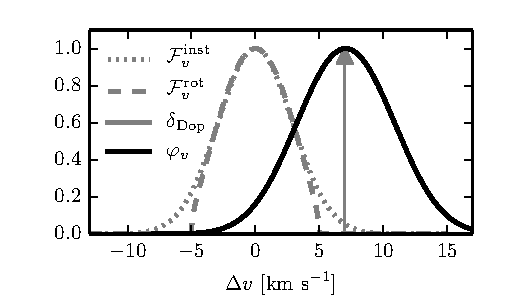
\includegraphics{figs/kernels.pdf}
  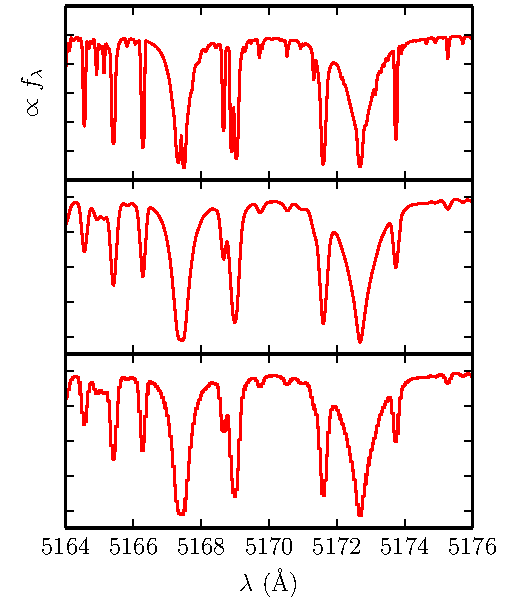
\includegraphics{figs/high2low.pdf}
  \caption{Panel 1: the instrumental (${\rm FWHM} =6.8\;\kms$) and rotational ($v \sin i = 5\;\kms$) broadening kernels, and their composite. Panel 2: A section of the raw, high resolution synthetic model at $R=$500,000. Panel 3: The spectrum after applying the composite broadening kernel, $\varphi_v$. Panel 4: The broadened spectrum downsampled to the pixels of the detector.}
\label{fig:broadening}
\end{center}
\end{figure*}

% SA: My idea for this figure is sort of 1-column wide (~3.5"), with a set of spectral panels going 
% down vertically.  The top panel shows a segment of the full resolution model.  The next one down 
% can show the individual kernels described above, as well as their composite, \varphi_v.  Then the 
% next panel down can show the convolved (but still full-resolution) spectrum.  Finally, the bottom 
% panel will show the spectrum re-sampled onto the observed pixels.  It need not be a large figure 
% (maybe 5" long?).

At this stage, the model is further modified in the flux dimension.  A typical synthetic spectrum 
is computed as the flux that would be measured {\it at the stellar surface}, and so needs to be 
diluted by the subtended solid angle, $\Omega = (R_{\ast}/d)^2$, where $R_{\ast}$ is the stellar 
radius and $d$ is the distance.  An additional wavelength-dependent scaling factor is applied to 
account for interstellar extinction, assuming a 
derived extinction law $A_{\lambda}$ \citep[e.g.,][]{cardelli89} that is parameterized by $A_V$.  
The parameters $\vt_{{\rm obs}, f} = [\Omega, \,\, A_V]$ are applied as
\begin{equation}
\vM(\vt) \equiv \vM(\vt_{\ast}, \vt_{\rm obs}) = \vM(\vt_{\ast}, \vt_{{\rm obs}, v}) \times \Omega \times 10^{-0.4\,A_{\lambda}},
\label{eqn:scaling}
\end{equation}
where we have simplified the notation by writing $\vt \equiv [\vt_{\ast}, \,\, \vt_{\rm obs}]$.

So far, the procedure summarized in Eq.~\ref{eqn:interp}-\ref{eqn:scaling} is composed of 
relatively straightforward operations demanded by practical astronomical and computing issues.  If 
the observed spectrum was {\it perfectly} calibrated, we could proceed to a likelihood calculation 
(Section~\ref{subsec:likelihood}) that makes a direct comparison with $\vM(\vt)$ at this point.  
However, that is unlikely to be the case.  The primary concern is that an imperfect calibration 
produces (presumably low-level) mismatches in the underlying shape of the observed spectrum on 
relatively broad wavelength scales.  When compared with the model, these mismatches might represent 
a non-trivial contribution to the likelihood, and thereby bias our estimates of the desired 
physical parameters.  Often, this concern is treated externally to any modeling procedure, usually 
by dividing the observed spectrum (and model spectrum) by an appropriate polynomial function.  But 
that ``normalization" procedure implicitly assumes that there is no relevant information content on 
those mismatched scales; if $\vt$ also contributes to the broad spectral shape, then adopting this 
approach will corrupt the inferences of these parameters.  Moreover, in practice this approach is 
limited, since defining an appropriate polynomial becomes difficult in cases where the spectral 
line density is high (e.g., molecular bands for cool stars).  

We adopt a somewhat analogous approach to deal with this issue, but cast it internal to the 
modeling framework to appropriately propagate the uncertainty introduced by additional degrees of 
freedom in the model.  The residual calibration errors are treated as an explicit contribution to 
the model spectrum, enabling us to explore the distribution of possible calibrations (see 
Section~\ref{subsec:MCMC}) and then eventually marginalize out the associated nuisance parameters.  
In essence, the inferences for the relevant stellar parameters will properly account for the 
underlying uncertainty in the calibration process.  This is achieved in practice by distorting the 
model spectrum with a (low-order) Chebyshev polynomial \citep[e.g.,][]{eisenstein06,koleva09}, 
\begin{equation}
\vM(\vt, \vT_{\rm cheb}) = \vM(\vt) \times \sum_n c_n \, T_n,
\end{equation}
where $T_n$ are the standard Chebyshev functions of order $n$ and the coefficients are treated as a
set of nuisance (hyper-)parameters, $\vT_{\rm cheb} = \{c_n\}^{\rm order}$, for each available 
spectral order in the dataset.  With judicious priors on $\vT_{\rm cheb}$, we can ensure that the 
unintended treatment of real spectral features (e.g., broad, deep molecular bands) as calibration 
artifacts is negligible (see Secton~\ref{sec:examples} for examples).  The lowest-order (scaling) 
coefficient, $c_0$, is by its nature degenerate with the solid angle parameter, $\Omega$.  
Therefore, we enforce an additional constraint by requiring that the mean of the polynomial is 
unity.  For data with a single spectral order, this means setting $c_0 = 1$.  If the goal is to 
model multiple spectral orders, we assign $c_0 = 1$ in an arbitrary order as an anchor, but permit 
the $c_0$ values in other orders to be different (as necessary).  It is worth noting that this 
formalism can, in principle, be extended to develop models for completely uncalibrated spectra, 
rather than the residual calibration mismatches as described here (with a suitable relaxation of 
the priors on $\vT_{\rm cheb}$).  Figure \ref{fig:cheb} offers a practical demonstration of how 
these nuisance parameters are applied. 
\comm{I envision this figure much like the previous one, in a 1-column vertical distribution of 
 panels.  At top, you would show the data spectrum at an overlap of two spectral orders, along 
 with the post-processed model with no Chebyshev polynomials applied.  Next, you would show the 
 two Chebyshev polynomials appropriate for the two orders.  And then in the final panel you would 
 revisit the top panel with the polynomials applied, demonstrating the improvement.}


\subsection{Model Evaluation \label{subsec:likelihood}}

The quality of the model spectrum is assessed by comparing to the data with a pixel-by-pixel 
likelihood calculation.  If we denote the data spectrum as $\vD$, then a corresponding 
$N_{\rm pix}$-dimensional residual spectrum can be defined for any input parameter set,
\begin{equation}
\vR \equiv \vR(\vt, \vT_{\rm cheb}) \equiv \vD-\vM(\vt, \vT_{\rm cheb}).
\end{equation}
To quantify the probability of the data conditioned on the model, we adopt a standard 
multi-dimensional Gaussian likelihood function,
\begin{equation}
p(\vD|\vM) =  \frac{1}{[(2 \pi)^{N_{\rm pix}} \det(\vC)]^{1/2}} \exp\left ( -\frac{1}{2}
   \vR^\trans \vC^{-1} \vR \right ), 
   \label{eqn:prob}
\end{equation}
which penalizes models that yield larger residuals and explicitly allows for covariances in the 
residual spectrum through the $N_{\rm pix} \times N_{\rm pix}$ matrix, $\vC$.  For practical 
numerical reasons, we generally consider the log-likelihood as the fit quality metric, which in 
this case is
\begin{equation}
  \ln{p(\vD | \vM)} = -\frac{1}{2} \left( \vR^\trans \vC^{-1} \vR + \ln{\det{\vC}} + N_{\rm pix} \ln{2\pi} \right).
  \label{eqn:lnprob}
\end{equation}

The covariance matrix $\vC$ characterizes both the measurement uncertainty ($\sigma$; 
``noise") in each pixel and the intrinsic covariance between pixels.  The special case where each 
pixel represents an independent measurement results in a diagonal covariance matrix, $\vC_{ij} = 
\delta_{ij} \,\, \sigma_i$ where $\sigma_i$ is the uncertainty in pixel $i$ and $\delta_{ij}$ is 
the Kronecker delta function, and Eq.~\ref{eqn:lnprob} reduces to the familiar
\begin{equation}
\ln{p(\vD | \vM)} = -\frac{1}{2} \sum_i^{N_{\rm pix}} \frac{\vR_i^2}{\sigma_i^2} \equiv -\frac{\chi^2}{2},
\label{eqn:chisq}
\end{equation}
the sum of the square of the residuals weighted by the inverse variances (squared uncertainties).  
However, the problem being addressed here necessitates the use of a more complex covariance matrix; 
additional off-diagonal terms that can explicitly characterize (1) pixel-to-pixel covariances 
imposed by the discrete over-sampling of the line-spread function, and (2) highly correlated 
residuals as manifestations of the still-imperfect model library are required to avoid biasing our 
inferences of the physically interesting parameters ($\vt$).  The following subsections describe 
how these issues are addressed in the practical implementation of $\vC$.  

\begin{figure*}[!htb]
\begin{center}
  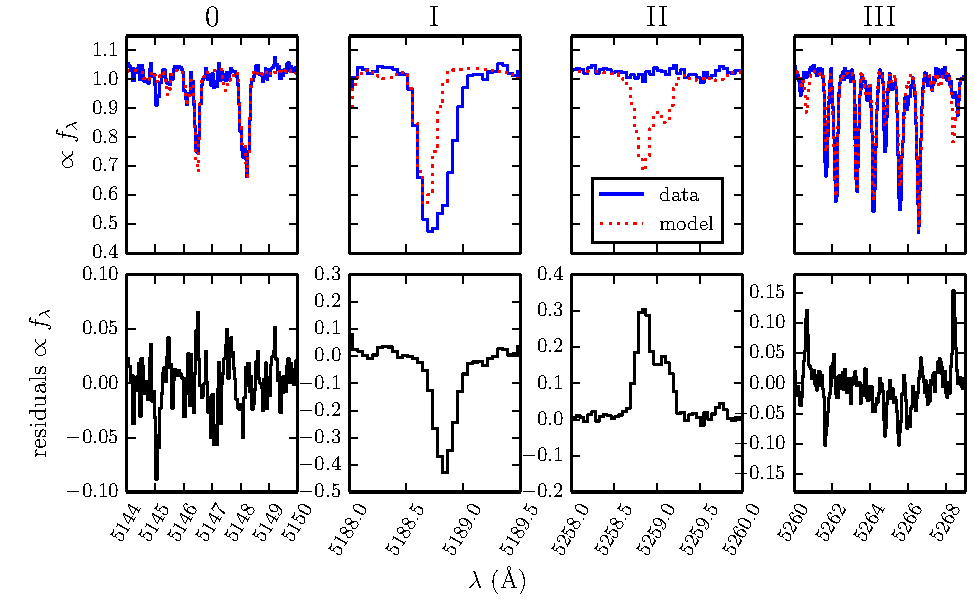
\includegraphics{figs/badlines.pdf}
  \caption{A collection of spectral lines which have imperfect model fits.
    From left to right: \textbf{Class 0} The majority of spectral lines
    ($\gtrsim 60$\%) will have minor differences in strength between data and
    model spectrum, which produce low-amplitude correlations in the residuals
    on the length scale of the width of a typical spectral line.  \textbf{Class
    I}: Sometimes ($\lesssim 5$\% of all lines), a missing opacity source in
    the model (in this case a line-blended \ion{Ca}{2}) leaves a large, highly correlated
    patch of negative residuals.  \textbf{Class II}: Sometimes ($\lesssim 5$\%
    of all lines), an extraneous line in the model leaves a large, highly
    correlated patch of positive residuals.  \textbf{Class III}: If the line strengths are
    substantially discrepant ($\lesssim 10$\% of all lines), there will be many
    correlated residuals of moderate amplitude.  The difficulty
    with class III lines is that for any specific line, there might exist a
    $\vtstar$ that will fit the line, but there does not exist a $\vtstar$ that
    will properly fit \emph{all} the lines.}
\label{fig:badlines}
\end{center}
\end{figure*}

\subsubsection{Global Covariance Structure}

Astronomical spectrographs are designed so that the detector over-samples the instrumental line 
broadening function with at least a few pixels.  Therefore, adjacent pixels are never completely 
independent samples of the observed spectrum.  In that case, a difference between an observed and 
modeled spectral feature will create a residual that spans multiple pixels.  This can be 
demonstrated in practice by examining the autocorrelation of the residual spectrum: a slight model 
mismatch will produce correlated residuals over a characteristic scale similar to the observational 
line-broadening kernel width.  Figure \ref{fig:class0} highlights a specific example of these 
correlated residuals in real data, where an imperfect model generates residuals which exhibit a 
significant autocorrelation signal on the scale of $\sim$4 pixels, which corresponds to the typical 
line width in this spectrum.  

\begin{figure*}[!htb]
\begin{center}
  $\vcenter{\hbox{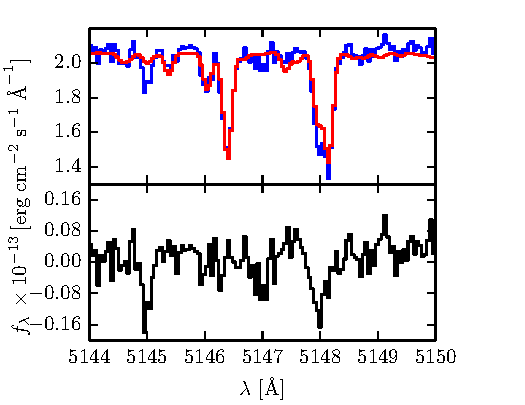
\includegraphics{figs/class0_residuals.pdf}}}$
  $\vcenter{\hbox{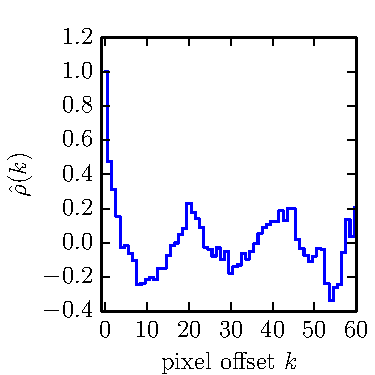
\includegraphics{figs/class0_autocorrelation.pdf}}}$
  \caption{\textbf{Left} The same low-amplitude, mildly covariant residuals from Figure~\ref{fig:badlines}, panel 0, but enlarged to show the mildly covariant structure produced by slight mismatch between the data and model spectra.   
  \textbf{Right} The autocorrelation (Equation~\ref{eqn:autocorrelation}) of the residual sequence shown at left. Notice that there is significant correlation for offsets of $\lesssim 4$ pixels.}
\label{fig:class0}
\end{center}
\end{figure*}

It seems important to distinguish here between ``noise" and the fit residuals.  Noise introduced to 
the spectrograph by astrophysical or instrumental effects is generally uncorrelated with 
wavelength.  The arrival of each photon to the detector is an independent event; while these 
photons are scattered by the instrumental line-spread function, the magnitude and direction of that 
scatter is independent for each such event.  In essence, the noise itself is uncorrelated, but the 
fit residuals likely are correlated.  However, from a mathematical perspective the correlated 
residuals can be treated in the same way as correlated noise, by constructing a non-trivial 
covariance matrix with off-diagonal terms.  In practice, this is achieved by parameterizing $\vC$ 
with a kernel that describes the covariance between any pair of pixels, representing wavelengths 
$\lambda_i$ and $\lambda_j$ (in many ways analogous to the standard two-point spatial correlation 
function used in cosmology).

For a well-designed spectrograph and sufficiently accurate model spectrum, this
{\it global} (i.e., present throughout the spectrum) covariant structure should
have a relatively low amplitude and small correlation length.  To describe that
structure, we assume a stationary covariance kernel (also called a radial basis
function) with an amplitude that depends only on the velocity distance between
two pixels, 
\begin{equation}
  r_{ij} = r(\lambda_i, \lambda_j) = \Delta v = \frac{c}{2} \left | \frac{\lambda_i 
   - \lambda_j}{ \lambda_i + \lambda_j} \right |,
\end{equation}
where $c$ is the speed of light.  The kernel is chosen to parametrically describe the covariance 
between pixel residuals, such that
\begin{equation}
  \mathcal{K}_{\rm g}(\lambda_i, \lambda_j) =  \langle \vR_i \; \vR_j \rangle.
  \label{eqn:expectation}
\end{equation}
A variety of kernels have been used in the field of Gaussian
processes to parameterize such a mildly covariant structure
\citep[e.g.,][]{rasmussen05}.  Here we adopt the \matern\ kernel with 
$\nu = 3/2$,
\begin{equation}
  \mathcal{K}_{\rm g}(\lambda_i, \lambda_j \, |\, a_{\rm g},\, \ell) = a_{\rm g} \left(1 + \frac{\sqrt{3}\, r_{ij}}{\ell} \right ) \exp 
   \left (- \frac{\sqrt{3}\, r_{ij}}{\ell} \right ),
\end{equation}
which is parameterized by an amplitude $a_g$ and scale $\ell$ and makes for a smooth transition to 
negligible covariance at large $r$.  To ensure that $\vC$ remains a relatively sparse matrix that 
enables computational expendiency, we employ a Hann window function
\begin{equation}
  w\,(\lambda_i, \lambda_j |\, r_0) = \left \{ 
    \begin{array}{cc}
    \frac{1}{2} + \frac{1}{2} \cos \left(\frac{\pi r_{ij}}{r_0} \right) & r_{ij} \le r_0 \\
    0 & r_{ij} > r_0 \\
  \end{array}
  \right .
  \label{eqn:Hann}
\end{equation}
to taper the kernel (so the effective kernel is $w \, \mathcal{K}_g$).  The truncation distance 
$r_0$ can be fixed to some reasonable multiple of the scale parameter (here we set $r_0 = 4\ell$).  
The examples in Figure \ref{fig:matern} demonstrate that such a kernel readily produces correlated 
structure in the residual spectrum that is similar to those seen in a typical data--model 
comparison.  

\begin{figure*}[!htb]
\begin{center}
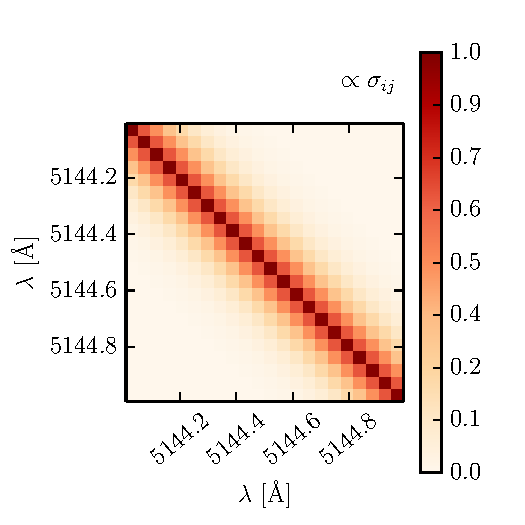
\includegraphics[width=0.4\textwidth]{figs/matern_matrix.pdf}
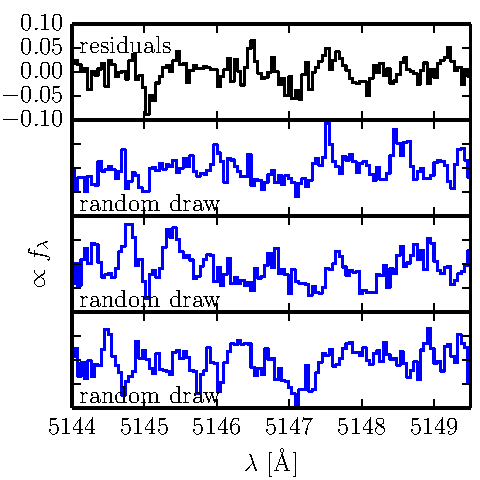
\includegraphics[width=0.4\textwidth]{figs/matern_draw.pdf}
\caption{\textbf{Left} Inset zoomed to show a small region of a typical covariance matrix, generated using the kernel in Equation~\ref{eqn:global} and common values for the hyperparameters. There is a small degree of covariance in elements within a few pixels off the diagonal, which quickly tapers off so that the majority of the matrix remains sparse ($\sigma_{ij} = 0$). This matrix is used to model a spectrum which is correlated on a $\sim$few pixel scale.
\textbf{Right} To demonstrate that this matrix properly models the correlated structure of the residuals, we compare the residuals to random residuals generated from a multivariate normal distribution with this covariance matrix. The top panel shows the same residuals shown in Figure~\ref{fig:class0}, and below are plotted three sets of simulated residuals. The amplitude and correlation length of the simulated residuals closely approximates the structure of the actual pixel residuals.}
\label{fig:matern}
\end{center}
\end{figure*}


\subsubsection{Local Covariance Structure}

Aside from the global covariance structure described above, there are likely also local regions of 
strong, highly correlated residuals that need to be treated in the modeling framework.  These large 
amplitude residual regions are usually produced by imperfect spectral lines in the models (e.g., 
missing opacity sources, uncertain oscillator strengths, etc.); some representative examples are 
highlighted in Figure \ref{fig:badlines}.  To parameterize such regions in the covariance matrix, 
we introduce a sequence of non-stationary kernels that explicitly depend on the actual wavelength 
values of a pair of pixels (on $\lambda_i$ and $\lambda_j$), and not simply the distance between 
them ($r_{ij}$).  

Assuming that these local residuals are produced primarily by pathological differences in the 
spectral line strength (rather than shape or center), a simple Gaussian is a reasonable residual 
model.  In that case, the $k^{\rm th}$ such local residual can be described as
\begin{equation}
\vR_{\lambda}(a_k, \mu_k, \sigma_k) = \frac{a_k}{\sqrt{2\pi}{\sigma_k}} \exp \left[ - \frac{r^2(\lambda,\mu_k)}{2\sigma_k^2} \right],
\end{equation}
with an amplitude $a_k$, a mean wavelength $\mu_k$, and a width $\sigma_k$.  Following 
Eq.~\ref{eqn:expectation}, the kernel that describes the covariance of any two pixels related to 
the $k^{\rm th}$ residual region is
\begin{equation}
  \mathcal{K}_k(\lambda_i, \lambda_j | a_k, \mu_k, \sigma_k) = \frac{1}{2\pi} \left(\frac{a_k}{\sigma_k}\right)^2 \exp \left [ - \, \frac{r^2(\lambda_i, \mu_k) + r^2(\lambda_j, \mu_k)}{2 \sigma_k^2}\right ].
\label{eqn:klocal}
\end{equation}
We again taper this kernel with a Hann window (Eq.~\ref{eqn:Hann}) to ensure computational 
efficiency with a sparse covariance matrix; in this case, the truncation distance $r_0$ can be set 
to some multiple of the Gaussian width (we set $r_0 = 4\sigma_k$).  
Figure \ref{fig:region} demonstrates how this non-stationary Gaussian 
kernel generates a localized region of enhanced variance that successfully mimics the kind of 
residuals produced by an inaccurate spectral line model.  In effect, these kernels down-weight the 
influence of such strong residuals in the likelihood calculation, mitigating any potential bias 
they might induce on inferences of the interesting parameters ($\vt$).  In essence, this is a 
robust, flexible, and unbiased method for (correlated) outlier rejection that preserves the 
integrity of the probabilistic framework being developed (as opposed to manual or threshold-based 
clipping/masking).  

These local kernels can be further modified to account for more complex residual structures.  For 
example, late-type stars with imperfectly modeled molecular bandheads may produce a complicated 
pattern of positive and negative residuals or a pronounced mismatch over a relatively large 
spectral scale.  This phenomenologically different local covariance behavior can still be treated 
in this framework, if we permit the kernel in Eq.~\ref{eqn:klocal} to be modified by another 
(stationary) function.  Here we assume that function is a squared exponential,
\begin{equation}
  \mathcal{S}_k(\lambda_i, \lambda_j |\, h_k) = \exp \left ( - \, \frac{r_{ij}^2}{2\,h_k^2}\right ),
\end{equation}
where $h_k$ is a bandwidth parameter; small $h_k$ generates high-frequency structure, and vice 
versa.  The functionality of this kernel modification (where the appropriate kernel is now $w_k \, 
\mathcal{S}_k \, \mathcal{K}_k$) is demonstrated for the worked example presented in Section 
\ref{subsec:mdwarf}.  
\comm{I have to admit that I do not really understand this very well.  I think some appropriate 
figures in Sect 3.2 will really help, though, so I'll wait for that before decided whether or not 
we need to change this part of the text.}


\subsubsection{Composite Covariance Matrix}

We can now compute the covariance matrix employed in the likelihood calculation 
(Eq.~\ref{eqn:lnprob}) as the linear combination of these kernels and the trivial pixel-by-pixel 
noise matrix, 
\begin{eqnarray}
\vC_{ij}(\vT_{\rm cov}) & = & b \, \delta_{ij}\sigma_i + \\ \nonumber
         &   &  w(r_{ij}|r_0 = 4\ell) \,\, \mathcal{K}_g(\lambda_i, \lambda_j|a_g, \ell) + \\ \nonumber
         &   &  \sum_k w(r_{ij}|r_0 = 4\sigma_k) \,\, \mathcal{S}_k(\lambda_i,\lambda_j | h_k) \,\, \mathcal{K}_k(\lambda_i, \lambda_j | a_k, \mu_k, \sigma_k),
\end{eqnarray}
where the covariance hyperparameters $\vT_{\rm cov} = [a_g, \ell, \{a_k, \mu_k, \sigma_k, 
h_k\}^{N_{\rm reg}}]$, $N_{\rm reg}$ is the number of local residual regions
(see below for details on how this is determined), and $b$ is assumed to be a
fixed parameter that scales up the pixel noise values to account for read
noise, noise added during the 2D to 1D spectral extraction procedure, and
interpolation uncertainties (see Section \ref{subsec:synthetic}; reasonable
values are $b \approx 1.02$--1.10 for well-calibrated optical spectra; see Section
\ref{sec:examples} for examples).  

\comm{No idea if this is your intention for $b$, but it was the only way I could rationalize it.}

\begin{figure*}[!htb]
\begin{center}
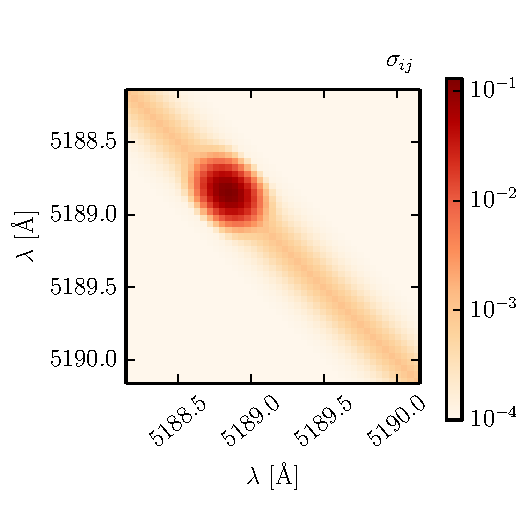
\includegraphics[width=0.4\textwidth]{figs/gauss_matrix.pdf}
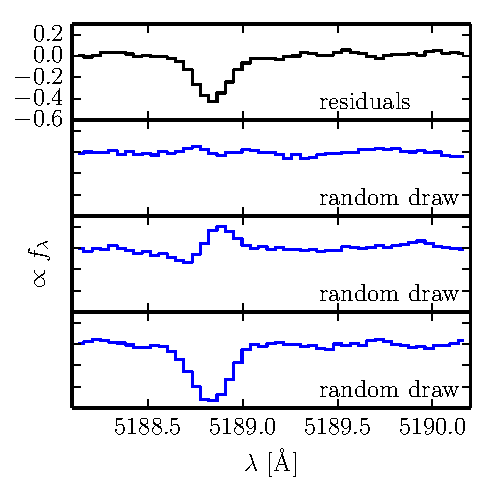
\includegraphics[width=0.4\textwidth]{figs/gauss_draw.pdf}
\caption{\textbf{Left} A typical covariance matrix including the Gaussian line kernel (Equation~\ref{eqn:line_total}). The same global covariance shown in Figure~\ref{fig:matern} is still present with the same hyperparameters, however now there is an additional patch of high covariance corresponding to the large, Gaussian-shaped residuals. These larger elements in the covariance matrix effectively down-weight the contribution of a poorly modeled synthetic spectral line.
\textbf{Right} The same spectroscopic residuals shown in Figure~\ref{fig:badlines}, class I, shown with three random draws from the covariance matrix. The random draws can take on a range of amplitudes--positive, negative, or even flat--because they are simply random draws that are described by the covariance matrix. The wide range of possible residual amplitudes match the structure and amplitude of the pixel residuals.}
\label{fig:region}
\end{center}
\end{figure*}


\subsection{Exploring the Posterior \label{subsec:MCMC}}

\comm{Not much done here...want to meet and discuss before I try editing.}

When iteratively fitting a spectrum (see \S\ref{subsec:MCMC}), we continue to add line covariance kernels until we have covered all of the high amplitude residuals. Typically, we will add line kernels until all residuals greater than three times the amplitude of the global covariance kernel are covered. In a single order of an echelle spectrum, there may be $N$ regions of high covariance that are parameterized by several line kernels (Equation~\ref{eqn:line}), which we group into an aggregate parameter $\vtlines = \{\vtline{1}, \vtline{2}, \ldots, \vtline{N}\}$. Along with the global covariance parameters and Chebyshev parameters for this order, we call the collection of nuisance hyperparameters for a specific order  (e.g., order $1$) $\vtorder{1} = \{\vtcheb, \vtglobal, \vtlines\}$. Taken together, the aggregated nuisance parameters for all of the $N$ orders are stored in $\vtorders = \{\vtorder{1}, \vtorder{2}, \ldots, \vtorder{N} \}$.

\todo{We can (should?) add an additional level to the hierarchy of
  hyperparameters and add parameters to describe the \emph{population
  characteristics} of poorly modeled spectral lines (mostly the typical width,
  amplitude of these lines).  This will tell us about the frequency and
distribution of spectral modelling errors.} 
We explicitly fit for the hyperparameters of the covariance kernels at the same
time we fit for the stellar parameters. While including these extra
parameters does increase the dimensionality and complexity of our model, they do provide several advantages. \emph{A priori} we do not know which
regions of the spectrum are improperly modeled. The covariance hyperparameters provide a framework to identify these regions iteratively and in a self-consistent manner. 

The traditional practice method of dealing with spectral mismatch is to simply mask out the regions of the spectrum which do not agree to within a certain tolerance.  Rather than arbitrarily excluding regions of the spectrum from the fit, these regions should instead be incorporated into in the fit with the appropriate weight. A model that includes covariance is far more likely than forcing the synthetic spectrum to fit perfectly, and far more flexible than arbitrarily masking regions which do not fit. The fitting procedure allows these weights to be determined self-consistently, such that lines which are slightly wrong can still bring information to bear on the stellar parameters. In fact, it may be the case that the lines that are off by a small amount (class 0 and III lines in Figure~\ref{fig:badlines}) actually provide the \emph{most information} about the stellar parameters, precisely because these lines are the most sensitive to stellar structure and consequentially are the most difficult to model correctly.

Another powerful benefit of including the covariance hyperparameters is the result of their ability to quantify and account for model-data mismatch. When a data spectrum is fit with a high-quality spectral library, the pixel residuals are less likely to be correlated, and the covariance structure will have a smaller amplitude and correlation length. This means that the inference on the stellar parameters will be more precise, in the same way that high quality data allows a more precise result. However, if the systematic mismatch between the data and model is large, then the hyperparameters will be larger and the precision of the stellar parameters will naturally inflate to respect the quality of model-data fit.

The benefits of using covariance hyperparameters extend beyond the use case of fitting a single stellar spectrum. If we fit many stars with the same set of synthetic models, we can use the structure of the covariance matrix to improve the models themselves (see \S\ref{subsec:learning}).


We use a Markov chain Monte Carlo (MCMC) algorithm coupled to a Gibbs sampler to explore the posterior distribution (Equation~\ref{eqn:lnprob}). The MCMC routine efficiently explores a high dimensional probability space using a stochastic, iterative approach. The Gibbs sampler provides a way to easily sample a large number of parameters in a simple, organized manner by sampling only a subset of parameters at any given time, but then rotating among all of the subsets of parameters. For more on MCMC and Gibbs samplers see \citet[ch 11]{gelman13} and the references therein. 

In addition to the stellar parameters $\vtstar$, we have introduced several nuisance parameters for calibration and residual modeling. These nuisance parameters have a logical hierarchical structure. At the lowest level of the hierarchy, a single order of an echelle spectrum has $N$ regions of high covariance $\vtlines = \{\vtline{1}, \vtline{2}, \ldots, \vtline{N}\}$. If we wish to evaluate the probability of the parameters of a specific line (e.g., line $1$) conditional on the current values of all other lines, then we denote this by $p(\vt_{\textrm{line} = 1} | \vt_{\textrm{lines} \ne 1})$. The collection of nuisance parameters for a specific order  (e.g., order $1$) is the aggregate parameter $\vtorder{1} = \{\vtcheb, \vtglobal, \vtlines\}$. Taken together, the aggregated nuisance parameters for all of the $N$ orders are stored in $\vtorders = \{\vtorder{1}, \vtorder{2}, \ldots, \vtorder{N} \}$. Because the nuisance parameters for a single echelle order are independent from the nuisance parameters for any other echelle order, we have $p(\vt_{\textrm{order} = 1} | \vt_{\textrm{orders} \ne 1}) = p(\vt_{\textrm{order} = 1})$. 

\begin{figure*}[!htb]
\begin{center}
  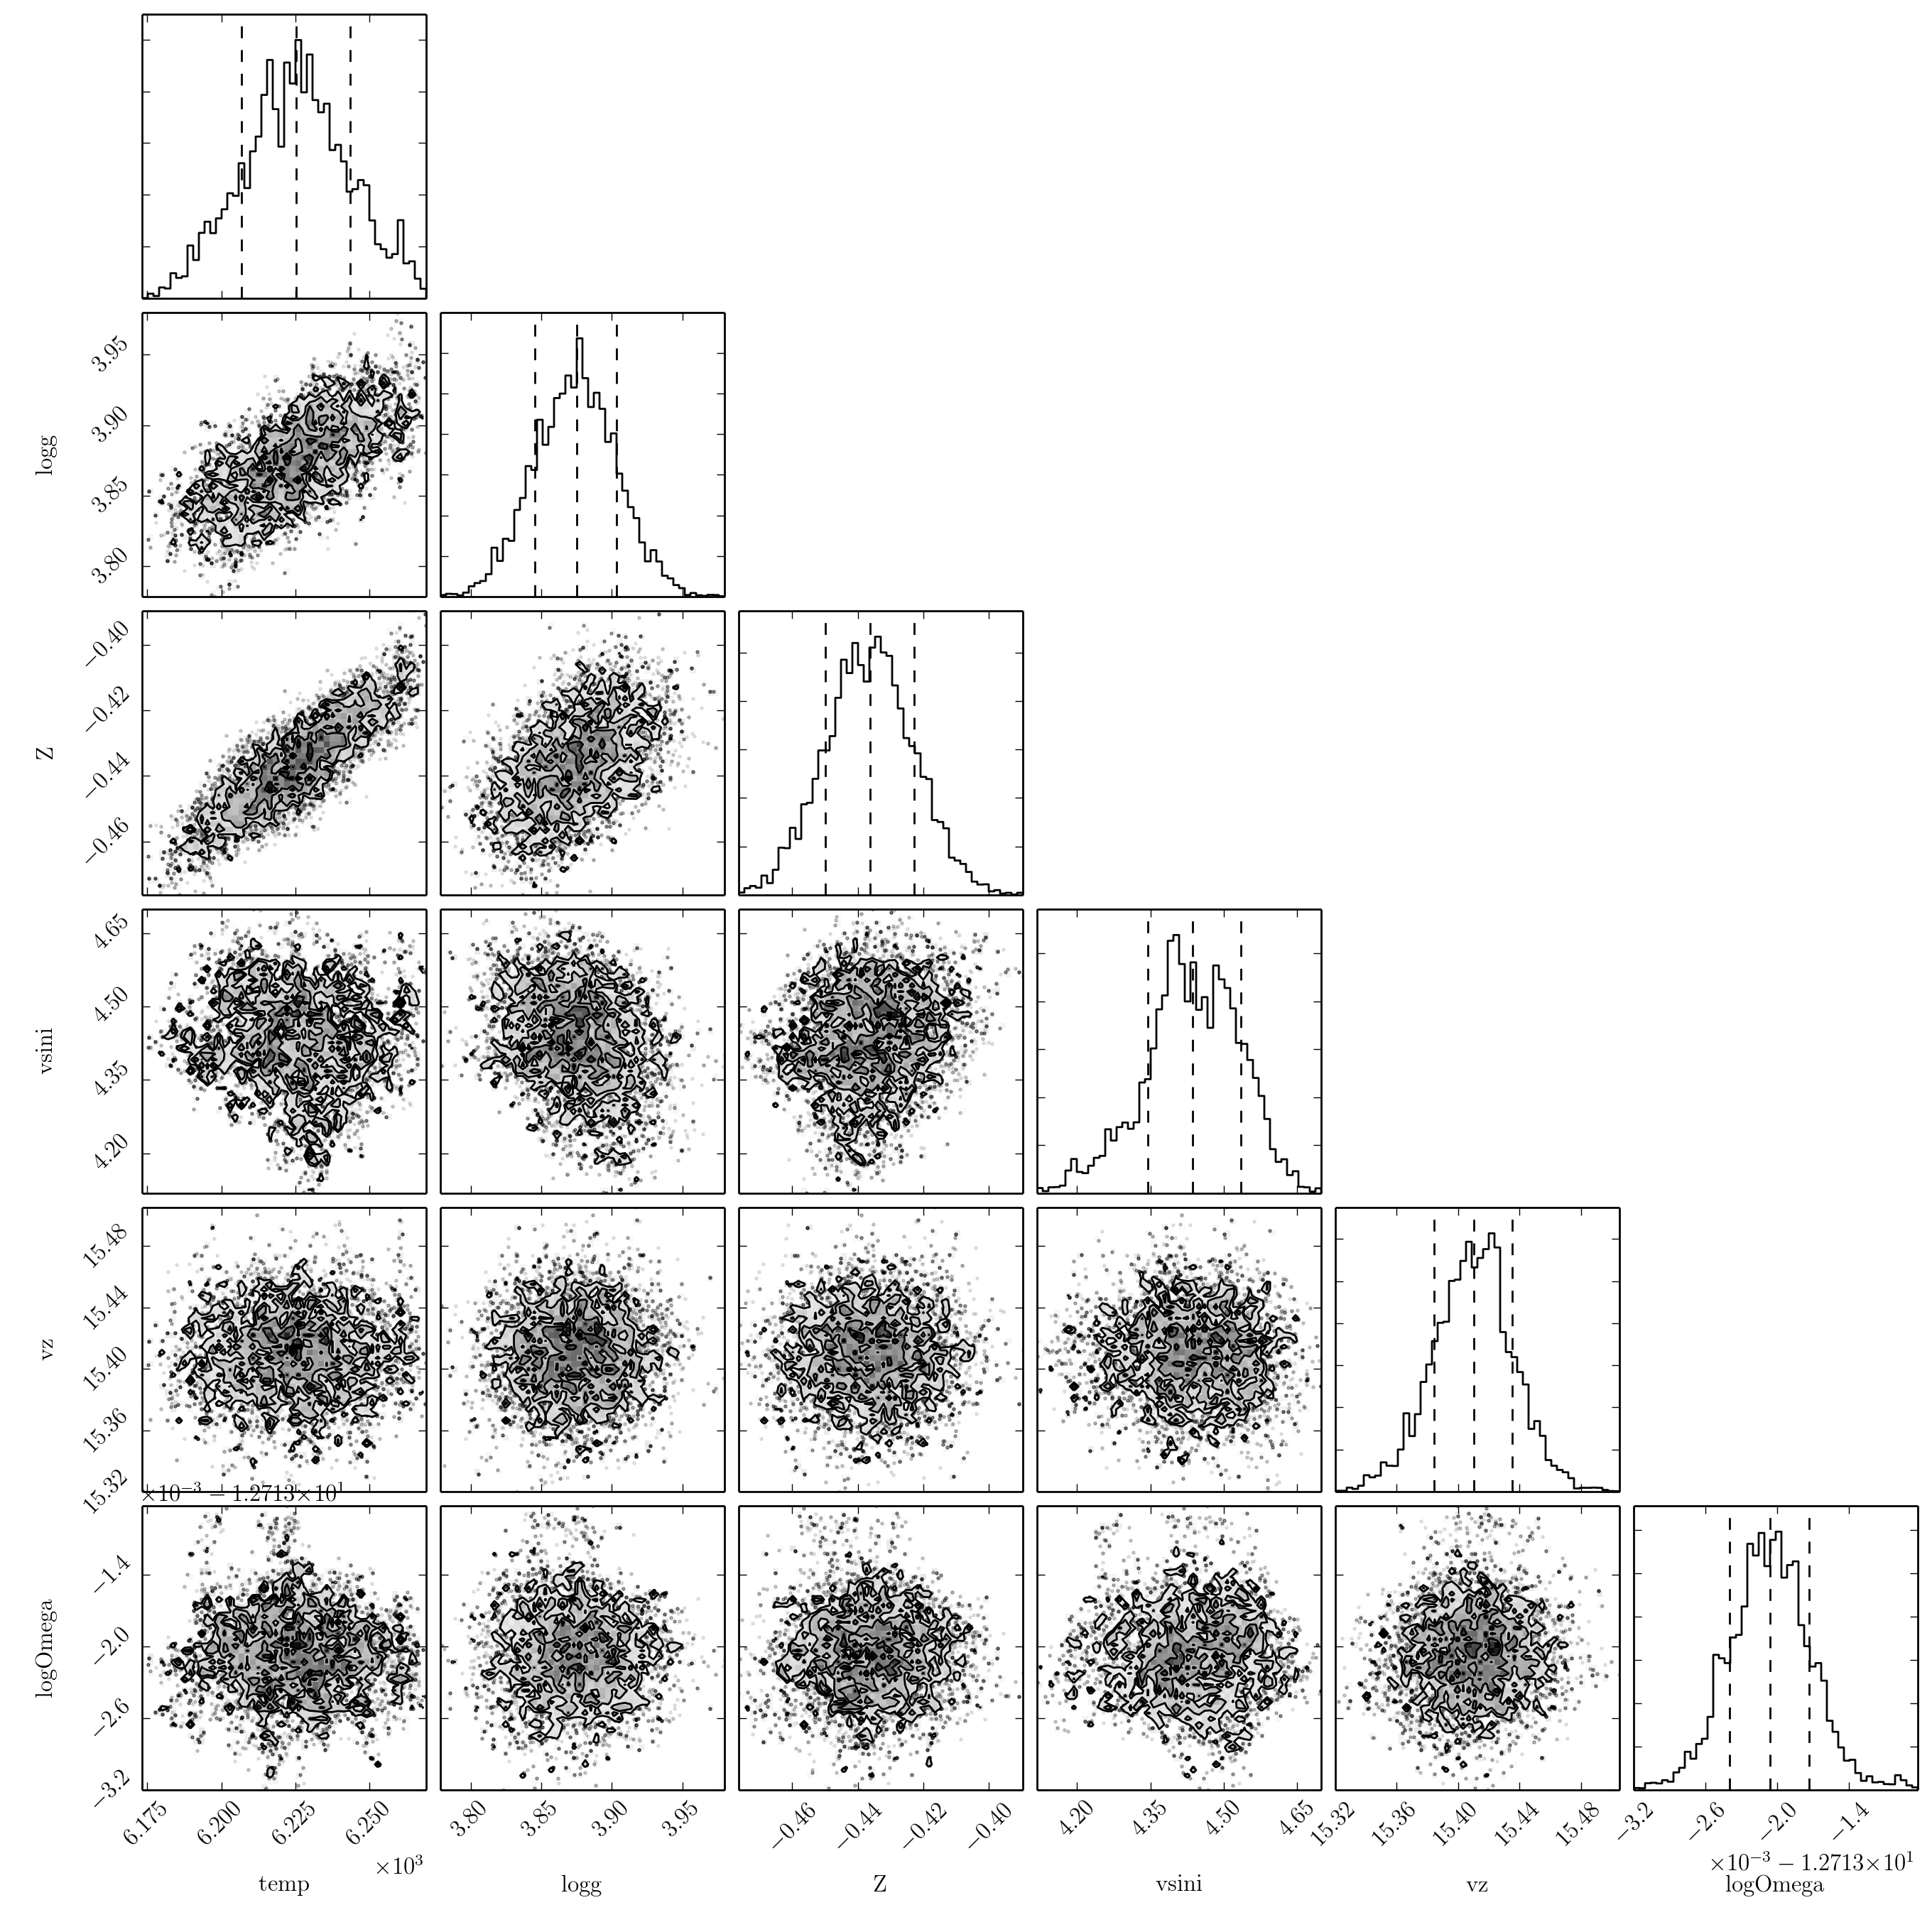
\includegraphics[draft, width=5in]{figs/stellar_triangle.png}
  \caption{The posterior probability function of the stellar parameters for WASP-14, an F star, as explored by the MCMC Gibbs sampler. These stellar parameters are marginalized over the Chebyshev and noise parameters. Figure generated with \texttt{triangle.py} \citep{foreman-mackey14}.
}
\label{fig:stellar_posterior}
\end{center}
\end{figure*}

\begin{figure*}[!htb]
\begin{center}
  \includegraphics[draft, width=3in, height=3in]{figs/global_posteriors.pdf}
  \includegraphics[draft, width=3in, height=3in]{figs/line_posteriors.pdf}
  \caption{\textbf{Left}: The posterior probability function of the global covariance parameters, as explored by the MCMC Gibbs sampler, marginalized over the stellar and line noise parameters. \textbf{Right}: The posterior probability function of the line parameters, marginalized over the stellar and global noise parameters.}
\label{fig:noise_posterior}
\end{center}
\end{figure*}

The Gibbs sampler iteratively explores this hierarchy of parameters. At each level of the hierarchy, corresponding to a different subset of nuisance parameters, we use the Metropolis-Hastings algorithm to propose a new subset of parameters and then either accept or reject them. This process of proposal and acceptance/rejection is called ``sampling.'' The Gibbs sampler rotates between sampling in different subsets of parameters, eventually sampling all of the nuisance parameters at a certain cadence. To initialize the MCMC algorithm, we make a reasonable guess for the starting parameters. We use existing spectral types in the literature for the stellar parameters, flat Chebyshev polynomials (no flux-calibration correction), and no covariance structure in the residuals (the global covariance parameters are set to zero and no line kernels are instantiated). We use superscripts to denote iterations of the MCMC algorithm. $i$ denotes the parameters from the current iteration and $i - 1$ denotes the previous iteration. The Gibbs sampler rotates among subsets of the parameters as follows 

\begin{enumerate}
  \item Sample in the stellar parameters. For each proposal of the Metropolis-Hastings algorithm, generate a model spectrum following the steps in \S\ref{subsec:postprocess}. When deciding whether or not to accept the parameters, the Gibbs sampler evaluates $p(\vtstar^i | \vtorders^{i-1})$.
  \item For each order of the echelle spectrum
    \begin{enumerate}
      \item Sample in the Chebyshev polynomial parameters. Adjust the spectrum as detailed in \S\ref{subsec:postprocess}.Gibbs sampler evaluates $p(\vtcheb^{i} | \vtstar^{i}, \vtglobal^{i -1}, \vtlines^{i-1})$.
      \item Sample in the global covariance parameters. Adjust the covariance matrix $C$ as described in \S\ref{subsec:covariance}. Gibbs sampler evaluates $p(\vtglobal^{i}| \vtstar^{i}, \vtcheb^{i}, \vtlines^{i -1})$.

      \item Check to see whether the algorithm should instantiate/delete new/old line kernels
      \item For each line kernel $k$
	\begin{enumerate}
	  \item Sample in the parameters for each line, conditional on the parameters for all the other lines. Adjust the covariance matrix $C$ as described in \S\ref{subsec:covariance}. Gibbs sampler evaluates $p(\vtline{k}^i| \vt_{\textrm{lines}\ne k}^{i - 1})$.
	\end{enumerate}
    \end{enumerate}
\end{enumerate}

At each stage of the Gibbs sampler, the likelihood function (Equation~\ref{eqn:lnprob}) is evaluated for a proposal of a particular subset of parameters, conditional on the current values of all the other parameters. This hierarchical parameter structure and the kernel parameterization of the covariance matrix influences how the algorithm may be efficiently implemented in code. For a typical optical spectrum with $\gtrsim$1,000 pixels, the most computationally intensive step of the likelihood evaluation is usually the matrix product $\fR^T C^{-1} \fR$. Since we have designed the covariance matrix to be sparse, we can use optimized sparse matrix algorithms which are much faster and memory efficient than dense matrix operations. Because we are not interested in the matrix inverse $C^{-1}$ by itself, but rather the product with the residual vectors, we can use efficient routines for solving linear systems to bypass the computationally difficult step of matrix inversion. Additionally, because the covariance matrix is positive semi-definite, we can use the Cholesky factorization of the matrix to optimize the evaluation of the matrix product. Once the covariance matrix is factorized, any subsequent evaluation of the matrix product for different residual vectors $\fR$ is extremely rapid. This makes the $\vtstar$ and $\vtcheb$ steps of the Gibbs sampler extremely fast.
When we sample in the nuisance parameters which affect the covariance matrix, we must redo the Cholesky factorization of $C$ for each update. However, because we designed the kernels to deliver a sparse matrix these operations are efficient enough to be used with an MCMC algorithm.  We use the high-performance \texttt{SuiteSparse/CHOLMOD}\footnote{\url{http://www.cise.ufl.edu/research/sparse/cholmod/}} library to implement the sparse matrix and Cholesky factorization operations \citep{chen08, davis09} and the Metropolis-Hastings sampler included in the \texttt{Python} MCMC package \texttt{emcee} \citep{foreman-mackey12}.

We run the MCMC Gibbs sampler for many iterations until the estimate of the posterior distribution has converged. To check that the chain is not stuck in a local maximum of the posterior, we redo the MCMC run many times with different starting parameters, to ensure that the algorithm converges to the same global maximum. A major advantage of using the MCMC algorithm to explore the multidimensional probability space is that it provides numerical samples in each dimension. Therefore, marginalizing out a parameter (i.e., numerically integrating over a dimension in probability space) is as simple as combining all of the samples in this dimension. This enables us to present a posterior of the stellar parameters $\vtstar$ (Figure~\ref{fig:stellar_posterior}) which has been marginalized over all of the nuisance hyperparameters. This posterior is the final estimate of the stellar parameters which \emph{incorporates} any inherent uncertainty due to model mismatch (via the covariance hyperparameters) and flux-calibration (via the Chebyshev polynomials).

The benefit of including nuisance parameters and then marginalizing over them is that we can self-consistently model the uncertainty inherent to any spectrum while naturally capturing any degeneracy between the model parameters. If stellar parameters are estimated using a method which ignores these nuisance parameters (e.g., by-eye fitting) and then the astronomer arbitrarily inflates the parameter uncertainties to reflect intuition, the degeneracy between parameters is artificially destroyed. This leads to estimates of stellar parameters with more uncertainty than necessary. 
\todo{Since this point is better carried with an example or test using the global covariance structure and not using it (see Test 1), we might want to defer this discussion to the testing section.}

\subsection{Applications}
\label{subsec:learning}
By cataloguing the covariance structure of the residuals, especially those generated from strong spectral line mismatch, we collect valuable information about the quality of the synthetic spectra. After fitting many stars, the accumulated knowledge of the data-model mismatch can be used when fitting a new star. The previous structure of the covariance matrix allows us to set priors on what the covariance in certain regions of the spectrum should be, which will speed convergence for this new star. Additionally, after fitting several stars, the average value of the covariance matrix will inform us about the quality of specific spectral lines in the synthetic models. 

Linking the covariance matrices of stars could be done serially, where the aggregate covariance matrix of all previous fits is used as a prior for the current iteration. Or, the covariance matrices could instead be linked hierarchically, in that the parameters describing the depth and width of a line residual for a specific star $a_1$ and $\sigma_1$, are modeled as coming from of a population of possible depths and widths for a given spectral type. Each stellar spectrum will have a slightly different realization of a spectral line, which will have some scatter about the average residual height. Linking the covariance matrix between spectra of similar stars allows us to grow more confident in our assessment that certain synthetic spectral lines are indeed outliers and should be appropriately down-weighted. In turn, as we become more certain of the weights, the stellar posteriors will become narrower and make our estimates of the stellar parameters more precise. This ability of the model to mutually inform sets of parameters is one of the major advantages of hierarchical Bayesian analysis \citep{kruschke10}.

Once determined, this average covariance matrix could be delivered to the communities that created the synthetic libraries, which would enable them to rapidly pinpoint and correct defects in the synthetic models. \todo{more delicate phrasing?} Alternatively, we could correct the models ourselves by using the chain of logic and mathematical post-processing that we used to created the synthetic model spectrum to reverse-engineer what the behavior of the raw synthetic spectrum \emph{should} be, at the raw $R \gtrsim$~100,000 resolution. This fundamental application of machine learning would enable us to create our own library of semi-empirical stellar models. Rather than simply assembling an empirical spectral library using only real stellar spectra, this combined approach is more powerful because the stellar atmospheres provide an actual anchor point of fundamental stellar parameters tied down by the laws of stellar physics.

\section{Worked Examples \label{sec:examples}}
Here are some ideas of which tests we might want to show.

\paragraph{Test 1}: Fitting with and without the global covariance kernel to show how the width of the posteriors nicely inflates to reasonable uncertainties.

\paragraph{Test 2}: I think we should fit both an F/G star (WASP-14) and a K/M star (TBD) with both the Kurucz and PHOENIX spectra. This will show a few things
\begin{itemize}
  \item Spectral parameters can vary by a large margin depending on which spectral library you use ($200~K$ or more).
  \item Both spectral libraries have stars that they perform better and worse on.
  \item This will be reflected in the increased level of global noise, and number of ``bad'' regions that have been instantiated.
\end{itemize}

\section{Discussion \label{sec:discussion}}

\section{Conclusion \label{sec:conclusion}}

\bibliographystyle{yahapj}
\bibliography{stellarspectra}

\appendix

\begin{table}[!htb]
\begin{tabular}{ll}
\hline
\hline
Symbol & Description\\
\hline
\hline
$i$ & index specifying a pixel\\
$\lambda_i$ & wavelength corresponding to a given pixel $i$\\
$\vg$ & fundamental stellar parameters, $T_{\rm eff}, \log(g), \Z, \A$\\
  & that parameterize a synthetic spectrum from the grid\\
$\vpp$ & stellar parameters $v \sin i$, $v_z$, $A_V$, and $R^2/d^2$ that\\
  & are applied during ``post processing'' of the synthetic spectrum\\
$\vtstar$ & $\{\vg,\vpp \}$\\
$\finst(\lambda)$ & data spectrum\\
$\fsynth(\lambda)$ & synthetic spectrum\\
$\vtcheb$ & the set of Chebyshev polynomial coefficients $\{c_0, c_1, \ldots, c_N\}$\\
$\vtline{1}$ & \\
$\vtlines$ & \\
$\vtorder{1}$ & \\
$\vtorders$ & \\
$\vt$ & the parameters $\{\vg, \vpp, \vN\}$ that completely describe a model spectrum\\
$\fDi$ & data flux for a given pixel, $D(\lambda_i)$\\
$\fD$ & data vector comprised of all $\fDi$, $i = \{1, \ldots, N\}$\\
$\fMi$ & model flux for a given pixel, $M(\lambda_i | \vt)$\\
$\fM$ & model vector comprised of all $\fMi$, $i = \{1, \ldots, N\}$\\
$\sigma_i$ & Poisson noise for a given pixel $i$\\
$R_i$ & residuals $\fDi - \fMi$\\
$\fR$ & residual vector $\fD - \fM$\\
$C$ & covariance matrix\\
$\sigma_{ij}$ & element in the covariance matrix\\
$r(\lambda_i, \lambda_j)$ & radial distance in wavelength space corresponding to $\Delta v$\\
$k_{\rm global}$ & global covariance kernel\\
$k_{\rm line}$ & regional covariance kernel\\
\hline
\end{tabular}
\caption{Nomenclature used in this document.}
\label{tab:nomenclature}
\end{table}

This version of the paper was generated
 from a git repository available at \url{http://github.com/iancze/StellarSpectra/}
 with git hash \texttt{\githash\,(\gitdate)}.



\end{document}
